\subsection{UC 16 - Telegram - Interazioni}

	\begin{figure}[H]
		\centering
		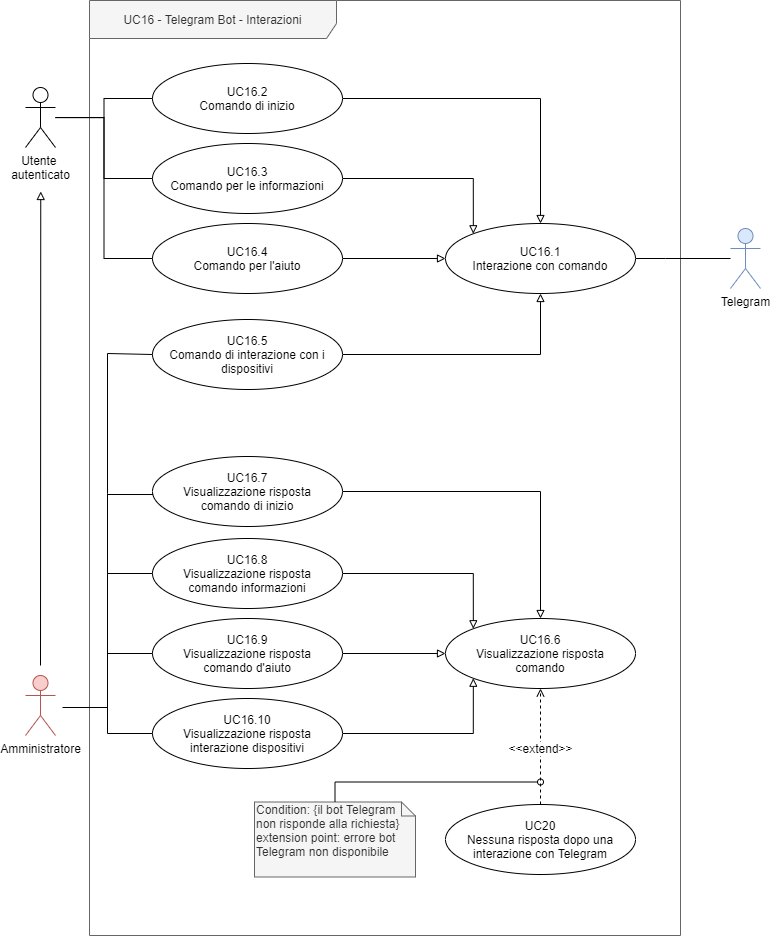
\includegraphics[scale=0.60]{res/images/uc16}
		\caption{Diagramma che descrive il processo di interazione con il bot tramite Telegram.}
	\end{figure}

	\begin{itemize}
		\item \textbf{attori primari:} utente autenticato, moderatore ente;
		\item \textbf{attori secondari:} \glock{Telegram};
		\item \textbf{descrizione:} l'utente mentre è nell'applicazione di \glock{Telegram} può eseguire delle interazioni per gestire dispositivi remoti nel sistema o ricevere informazioni particolari;
		\item \textbf{precondizione:} l'utente sta usando l'applicazione di \glock{Telegram} e ha eseguito l'autenticazione;
		\item \textbf{postcondizione:} l'utente riceve un messaggio di risposta dal \glock{bot} di \glock{Telegram};
		\item \textbf{scenario principale:}
		\begin{enumerate}
			\item l'utente esegue una interazione con il \glock{bot} di \glock{Telegram}.
		\end{enumerate}
	\end{itemize}

	\subsubsection{UC 16.1 - Interazione con comando}

	\begin{itemize}
		\item \textbf{attori primari:} utente autenticato, moderatore ente;
		\item \textbf{attori secondari:} \glock{Telegram};
		\item \textbf{descrizione:} l'utente esegue una interazione con \glock{Telegram} e riceve una risposta in base al comando che ha inviato;
		\item \textbf{precondizione:} l'utente sta usando l'applicazione di \glock{Telegram};
		\item \textbf{postcondizione:} l'utente riceve un messaggio di risposta dopo aver eseguito una interazione con \glock{Telegram};
		\item \textbf{scenario principale:}
		\begin{enumerate}
			\item l'utente sta usando l'applicazione di \glock{Telegram} e ha una chat aperta e autenticata con il bot;
			\item l'utente esegue una interazione con \glock{Telegram};
			\item l'utente riceve dei messaggi di risposta da parte del \glock{bot} di \glock{Telegram};
		\end{enumerate}
		\item \textbf{specializzazioni:}
		\begin{itemize}
			\item comando di inizio (UC16.2);
			\item comando per le informazioni (UC16.3);
			\item comando per l'aiuto (UC16.4);
			\item comando di interazione con i dispositivi (UC16.5).
		\end{itemize}
	\end{itemize}

	\subsubsection{UC 16.2 - Comando di inizio}

	\begin{itemize}
		\item \textbf{attori primari:} utente autenticato;
		\item \textbf{attori secondari:} \glock{Telegram};
		\item \textbf{descrizione:} l'utente esegue una interazione con il comando di inizio per recuperare le informazioni sull'autenticazione;
		\item \textbf{precondizione:} l'utente sta usando l'applicazione di \glock{Telegram};
		\item \textbf{postcondizione:} l'utente ha eseguito una interazione con \glock{Telegram};
		\item \textbf{scenario principale:}
		\begin{enumerate}
			\item l'utente sta usando l'applicazione di \glock{Telegram};
			\item l'utente invia il comando.
		\end{enumerate}
	\end{itemize}


	\subsubsection{UC 16.3 - Comando di informazioni}

	\begin{itemize}
		\item \textbf{attori primari:} utente autenticato;
		\item \textbf{attori secondari:} \glock{Telegram};
		\item \textbf{descrizione:} l'utente esegue una interazione con il comando di \textit{informazioni} per recuperare la versione del bot, le info del sistema e l'account con cui si è autenticati;
		\item \textbf{precondizione:} l'utente ha iniziato a interagire con \glock{Telegram};
		\item \textbf{postcondizione:} l'utente ha eseguito una interazione con \glock{Telegram};
		\item \textbf{scenario principale:}
		\begin{enumerate}
			\item l'utente sta usando l'applicazione di \glock{Telegram};
			\item l'utente invia il comando.
		\end{enumerate}
	\end{itemize}



	\subsubsection{UC 16.4 - Comando per l'aiuto}


	\begin{itemize}
		\item \textbf{attori primari:} utente autenticato;
		\item \textbf{attori secondari:} \glock{Telegram};
		\item \textbf{descrizione:} l'utente esegue una interazione con il comando di \textit{aiuto} per recuperare la lista dei comandi disponibili;
		\item \textbf{precondizione:} l'utente ha iniziato a interagire con \glock{Telegram};
		\item \textbf{postcondizione:} l'utente ha eseguito una interazione con \glock{Telegram};
		\item \textbf{scenario principale:}
		\begin{enumerate}
			\item l'utente sta usando l'applicazione di \glock{Telegram};
			\item l'utente invia il comando.
		\end{enumerate}
	\end{itemize}


	\subsubsection{UC 16.5 - Comando di interazione con i dispositivi}

	\begin{itemize}
		\item \textbf{attori primari:} moderatore ente;
		\item \textbf{attori secondari:} \glock{Telegram};
		\item \textbf{descrizione:} l'utente esegue una interazione per inviare un input testuale ad un dispositivo attivo;
		\item \textbf{precondizione:} l'utente ha iniziato a interagire con \glock{Telegram} e l'utente è autenticato come Moderatore ente.
		\item \textbf{postcondizione:} l'utente ha eseguito una interazione con \glock{Telegram};
		\item \textbf{scenario principale:}
		\begin{enumerate}
			\item l'utente sta usando l'applicazione di \glock{Telegram};
			\item l'utente invia il comando.
		\end{enumerate}
	\end{itemize}

%%%%%%%%%%%%%%%%%%%%%%%%%%%%%%%%%%%%%%%%%%%%%%%%%%%%%%%%%%%%%%%%%%%%%%%%%%%%%%%%%%%%%%%%%%%%

	\subsubsection{UC 16.6 - Visualizzazione risposta comando }

	\begin{itemize}
		\item \textbf{attori primari:} utente autenticato;
		\item \textbf{attori secondari:} \glock{Telegram};
		\item \textbf{descrizione:} l'utente riceve un messaggio di ritorno su \glock{Telegram}, dopo aver inviato il comando;
		\item \textbf{precondizione:} l'utente ha iniziato a interagire con \glock{Telegram} e l'utente è autenticato come Moderatore ente;
		\item \textbf{postcondizione:} l'utente ha eseguito una interazione da \glock{Telegram};
		\item \textbf{scenario principale:}
		\begin{enumerate}
			\item l'utente riceve un messaggio dal \glock{bot} di \glock{Telegram}.
		\end{enumerate}
		\item \textbf{estensioni:}
		\begin{itemize}
			\item nessuna risposta dopo una interazione con Telegram (UC 20);
		\end{itemize}
		\item \textbf{specializzazioni:}
		\begin{itemize}
			\item visualizzazione risposta comando di inizio (UC16.7);
			\item visualizzazione risposta comando informazioni (UC16.8);
			\item visualizzazione risposta comando d'aiuto (UC16.9);
			\item visualizzazione risposta interazione dispositivi (UC16.10).
		\end{itemize}
	\end{itemize}

	\subsubsection{UC 16.7 - Visualizzazione risposta comando di inizio }

	\begin{itemize}
			\item \textbf{attori primari:} utente autenticato;
			\item \textbf{attori secondari:} \glock{Telegram};
			\item \textbf{descrizione:} l'utente riceve un messaggio di ritorno su \glock{Telegram}, dopo aver inviato il comando, illustrando le informazioni dell'account autenticato;
			\item \textbf{precondizione:} l'utente sta usando l'applicazione di \glock{Telegram};
			\item \textbf{postcondizione:} l'utente ha eseguito una interazione da \glock{Telegram};
			\item \textbf{scenario principale:}
			\begin{enumerate}
				\item l'utente riceve un messaggio al \glock{bot} di \glock{Telegram}.
			\end{enumerate}
		\end{itemize}

	\subsubsection{UC 16.8 - Visualizzazione risposta comando informazioni}

	\begin{itemize}
			\item \textbf{attori primari:} utente autenticato;
			\item \textbf{attori secondari:} \glock{Telegram};
			\item \textbf{descrizione:} l'utente riceve un messaggio di ritorno su \glock{Telegram}, dopo aver inviato il comando, illustrante la versione del bot, le info del sistema e l'account con cui si è autenticati;
			\item \textbf{precondizione:} l'utente ha iniziato a interagire con l'applicazione di \glock{Telegram};
			\item \textbf{postcondizione:} l'utente ha eseguito una interazione da \glock{Telegram};
			\item \textbf{scenario principale:}
			\begin{enumerate}
				\item l'utente riceve un messaggio dal \glock{bot} di \glock{Telegram}.
			\end{enumerate}
		\end{itemize}

	\subsubsection{UC 16.9 - Visualizzazione risposta comando d'aiuto }

	\begin{itemize}
			\item \textbf{attori primari:} utente autenticato;
			\item \textbf{attori secondari:} \glock{Telegram};
			\item \textbf{descrizione:} l'utente riceve un messaggio di ritorno su \glock{Telegram}, dopo aver inviato il comando, illustrante la lista dei comandi disponibili con una relativa descrizione;
			\item \textbf{precondizione:} l'utente ha iniziato a interagire con l'applicazione di \glock{Telegram};
			\item \textbf{postcondizione:} l'utente ha eseguito una interazione da \glock{Telegram};
			\item \textbf{scenario principale:}
			\begin{enumerate}
				\item l'utente riceve un messaggio dal \glock{bot} di \glock{Telegram}.
			\end{enumerate}
		\end{itemize}


	\subsubsection{UC 16.10 - Visualizzazione risposta interazione dispositivi}

		\begin{itemize}
			\item \textbf{attori primari:} moderatore ente;
			\item \textbf{attori secondari:} \glock{Telegram};
			\item \textbf{descrizione:} l'utente riceve un messaggio di ritorno su \glock{Telegram}, dopo aver inviato il comando, che segnala l'invio corretto dell'input al dispositivo;
			\item \textbf{precondizione:} l'utente ha iniziato a interagire con l'applicazione di \glock{Telegram} e ha inviato un comando;
			\item \textbf{postcondizione:} l'utente ha eseguito una interazione da \glock{Telegram};
			\item \textbf{scenario principale:}
			\begin{enumerate}
				\item l'utente riceve un messaggio dal \glock{bot} di \glock{Telegram}.
			\end{enumerate}
		\end{itemize}
